\chapter{Survey}
\label{chp:amtsurvey} 

To be able to map to what extent people care and are aware of their Facebook settings, regarding privacy, security and interdependent privacy, we designed and distributed a survey. The survey addressed the different settings available on Facebook, and awareness regarding Facebook applications and knowledge about interdependent privacy. For the design of the survey, we utilized SurveyMonkey which provides web-based survey solutions (See section \ref{sec:sm}). We distributed the survey on two platforms, namely Amazon Mechanical Turk (AMT) and Facebook. Amazon Mechanical Turk is a Internet marketplace where human intelligence is utilized to perform various tasks \cite{amazonweb}. For more information about Amazon Mechanical Turk, see section \ref{sec:amt}. To reach out to a even larger audience, we posted the survey-link on our Facebook pages. In this chapter we will describe how we designed and distributed our survey. We will examine the results with focus on interdependent privacy. 


\section{Constructing the Survey}
There is not much research on the area of interdependent privacy. To be able bring forward information and contribute to new research, we created a survey. When making the questions, we wanted to create an image of peoples use of Facebook, how they set their settings and how they know and care about their privacy and to what extent their privacy is dependent on other users. We quickly chose to use AMT as a platform for distributing the survey, because we wanted to create an image of the average Facebook user as well as getting a high diversity among the respondents (different countries, age, education etc.). Previous research shows positive results with the use of AMT \cite{expectations,incentivesAmt}. 

\paragraph{}
We started implementing the survey inside the survey template provided by AMT. After some consideration, we found that AMT did fulfil our requirements for the design, so we chose to implement the survey using SurveyMonkey instead. When creating the survey, we thought that it would be better to include some extra questions, than to leave some behind. When the survey first got distributed, we were not longer able to edit the questions. We therefore chose to include questions not only regarding privacy and interdependent privacy, but also other aspects of Facebook usage. For example some questions about security settings, usage, personal experience in regard of photos and comments sharing.

\subsection{Design}
AMT offers a template for creating surveys. This template uses HTML. It is simple, but requires more work from the requester. We found the template to be little user friendly, and it did not give you many design options. Our survey consist of many questions, and some of them had follow-up questions requiring text answers. It was then desirable to have these on two different pages. We did not want the respondents to have their answers affected by the next question. It requires more of the respondent to write a text answer, so to avoid them answering based on the next question we separated the questions onto different pages. For example, we have one question asking whether or not the use of Facebook has lead to any uncomfortable situations. If the user answers "Yes", a follow-up question asking to describe the situation that occurred will appear. If the user answers "No" the follow-up question will be skipped. If the user had seen the follow-up question, he/she may not be bothered to answer yes even though this may be the truthful answer. We did not find an easy solution to implement this design feature in AMT, so we looked for other options. Even though AMT provide their own "Survey"-template, they also provide a "Survey Link"-template. This means that you can create the survey somewhere else, and just link to it in AMT. We chose the latter, and used SurveyMonkey to create the survey. SurveyMonkey provided us with the tools and features necessary to design our survey as desired. 

\paragraph{Features we used in SurveyMonkey.}
SurveyMonkey offers several features, and has a intuitive user interface. It was easy to implement the questions, and separate them on different pages which was of high value to us. SurveyMonkey offers the ability to customize the appearance (color/theme, layout, etc.) of the survey to a higher extent than AMT. We put in a picture of the university logo, to emphasize the seriousness of the survey, as shown in \fref{fig:frontpage}. SurveyMonkey also offers many different question types (multiple choice, text box, matrix and drop-down menus, etc.), and restrictions on the questions. It was important to have some restrictions especially on the text boxes. Some of the restrictions that we used was limit the amount of characters in the text boxes, to avoid too long answers. We also made almost all questions mandatory, meaning that the respondents had to answer them before being able to move to next question. As mentioned we divided the questions onto several different pages. This gives the respondents the impression that the survey is shorter. Each page has a title on top, grouping the different areas the questions consider. A progress bar was added to show in percent how far into the survey the respondent is at any time. This gives a good overview, and the user get a feeling of how much is left. We chose to use these features to avoid overwhelming the respondents with too many questions at a time. 

SurveyMonkey offers a great user interface also when it comes to reviewing the answers. It is possible to see graphs showing the distribution of answers to all the questions, as well as individual answers. SurveyMonkey also offers a filter and comparing feature, which made the analysis a lot easier, especially when having a large number of respondents. 

\subsection{How the Survey is Structured} 
The first page seen when taking the survey, is a introduction page that shortly explains what the survey is about, and it's purpose. This page emphasizes the seriousness of the survey. When people see that it is a research survey carried out by master students at an University, we believe people will answer in a serious manner. The front page also includes the requirement for taking the survey, and a short explanation on where to find answers requested in some of the questions. This is shown in \fref{fig:frontpage}. As mentioned before, we have divided the questions into different areas, and we will now go through each area and emphasize and elaborate the questions we consider as most relevant and important. 
 
\begin{figure}[h!]
\centering
\fbox{
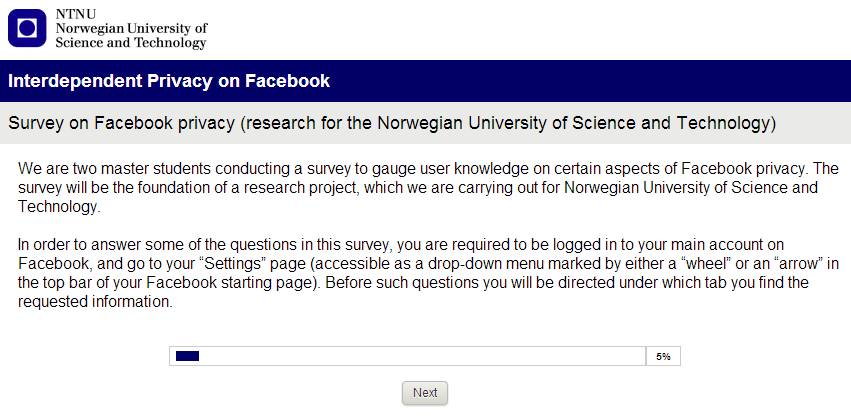
\includegraphics[width=1\textwidth]{firstpagesurvey.png} }
\caption[Front page of the survey]{\textbf{Front page of the survey.} This figure shows the first page of our survey. It gives a short explanation about the purpose of the survey, and what it concerns. It also give some helping guidelines to where to find answers to some of the questions, and the requirement for taking the survey (that you need to be logged in to your main Facebook account).} 
\label{fig:frontpage}
\end{figure}

\subsubsection{Facebook usage}
Following the first page is one page about Facebook usage. This page includes questions about sign-up year, how often they check their Facebook page and number of friends. 

\subsubsection{Facebook privacy: settings}
This is a part of the survey where the users need to be logged in to their main account on Facebook to check how their privacy settings look. The questions are taken directly from the "Privacy"-settings and "Timeline and tagging"-settings on Facebook. We divided these questions onto 4 different pages. Before we started asking about specific settings, ask the user how often they have checked their Facebook privacy settings during the last year.  One of the following pages ask for the privacy settings, and the other for the timeline and tagging settings. These questions are straightforward for the user, since all they have to do is to render the settings they have set themselves. This will easily show us how many that actually have checked their settings, and to what extent they have made them more, or less, private than default. At the end ask the user whether or not they consider changing their settings after having reviewed them. This can make for some interesting observations, and can also give an impression of whether or not the users care or are aware of the settings. 

\subsubsection{Facebook privacy: personal experience}

\begin{figure}[h!]
\centering
\fbox{
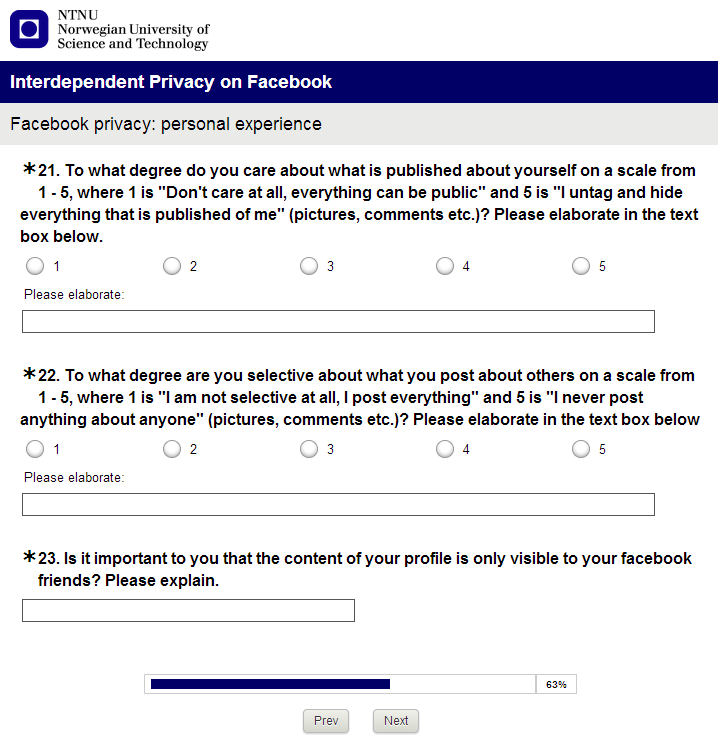
\includegraphics[width=1\textwidth]{page12.png} }
\caption[Question 21 and question 22 in the survey]{\textbf{Question 21 and question 22 in the survey.} This figure shows question 21 and 22 in the survey. The questions concerns to what degree (on a scale from 1 to 5) the respondents care about what is published about themselves, and what they publish about others. After each of the two questions it is a text box where the respondents can elaborate.} 
\label{fig:page12}
\end{figure}

This group of questions focus on the users personal experience with concern to both privacy and interdependent privacy. We ask whether or not the respondents have experienced that their use of Facebook has affected their professional life or led to any uncomfortable situations. Both of these questions have a follow-up question where to are asked to describe the situation that occurred. You will only be sent to the page with the follow-up question if you answered yes. If you answered no, you will skip the page with follow-up question. 

A big part of Facebook consists of sharing photos and comments with others, we therefore asked the respondents to indicate on a scale from 1 to 5 how much they care about what is published about themselves, and what they publish about others, see \fref{fig:page12}. It was mandatory for the users to give an answer on the scale. We added a text box for the users to elaborate if desired, but this was not mandatory. We received a total of 250 responses on our survey, and 190 of them chose to elaborate. 

\subsubsection{Facebook privacy: apps}
This is the part that concerns interdependent privacy (see section \ref{sec:intpriv}), and this is a very important part of our survey. As mentioned before this is a relatively unknown term, so we wanted to find out whether or not the respondents knew the meaning of interdependent privacy. Since the app platform on Facebook to a high extent relies on information about a user's friends, it is in this area interdependent privacy becomes more important to address. When you install an app on Facebook, it asks for your basic information, and often more information about you and your friends. For more detailed information about the app-platform see subsection \ref{subsec:app}. Question 26, 27, 28 and 29 (see \fref{fig:page14} and \fref{fig:page15}) asks about the users awareness regarding what kind of information the apps can retrieve. There exists settings directed towards apps on Facebook (see \fref{fig:apps2013}). In question 30 (\fref{fig:page15}) we ask the user to look at one of the app settings, "Apps others use". In this setting the user decides which information they make available to apps others use, in other words control the categories of information that people can bring with them when they use apps. We want to know if the user are aware of the existence of this settings. We did not ask for more specifics about what information they share, because this is not relevant. What is relevant is whether or not they know it exists, and are aware of what kind of information they share. We finish this part of the survey with the same question we started it with, if they know the meaning of interdependent privacy. We wanted to ask again to see if they got a higher understanding of the term after answering questions about apps, and saw how it is all interconnected. 

\begin{figure}[h!]
\centering
\fbox{
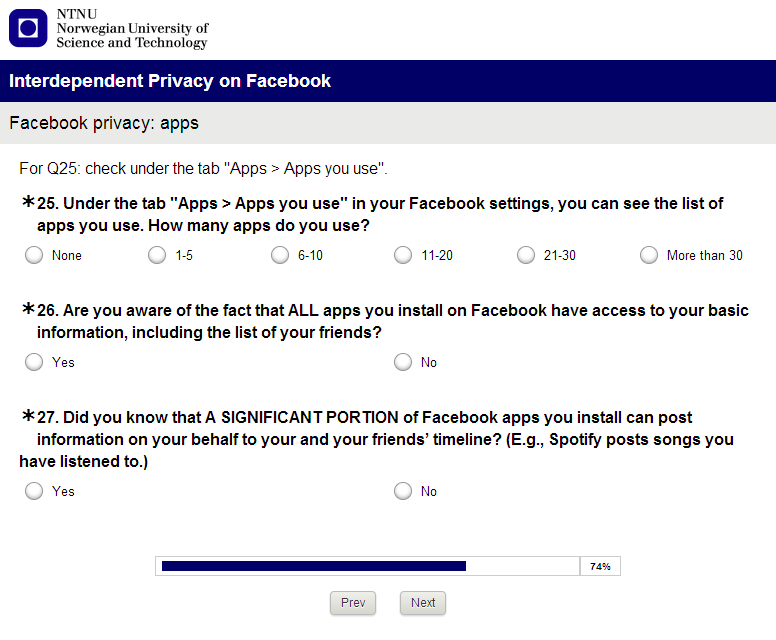
\includegraphics[width=1\textwidth]{page14.png} }
\caption[Question 25, 26 and 27 in the survey]{\textbf{Question 25, 26 and 27 in the survey.} This figure show question 25, 26 and 27 in our survey. Question 25 concern the number of apps the respondents use. Question 26 and 27 concerns the user's awareness connected to apps on Facebook.} 
\label{fig:page14}
\end{figure}

\begin{figure}[h!]
\centering
\fbox{
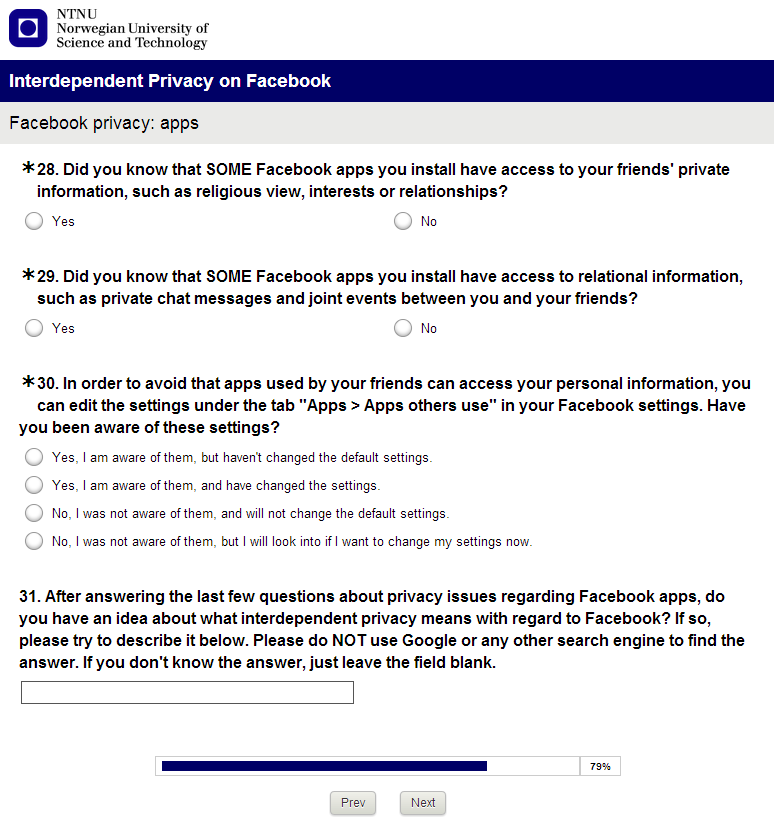
\includegraphics[width=1\textwidth]{page15.png} }
\caption[Question 28, 29, 30 and 31 in the survey]{\textbf{Question 28, 29, 30 and 31 in the survey.} This figure show question 28, 29, 30 and 31 in our survey. Question 28, 29 and 30 concerns the user's awareness connected to apps on Facebook. Question 31 asks the respondents whether or not they know what the term interdependent privacy means.} 
\label{fig:page15}
\end{figure}

\subsubsection{Facebook security: settings}
The main focus in this report is on privacy, not security. At the same time, we wanted to ask a few questions regarding Facebook security settings as well. The reason for this, is because we wanted to see if there was a connection between strict security settings and strict privacy settings among the respondents of our survey. The questions concern if the respondents use secure browsing and login notification.

\subsubsection{Demographics}
The last part of the survey, we have asked for demographic information about the respondents, to get a hunch of what kind of people have taken the survey. We chose to put the demographics part at the end, rather than in the beginning. We assume that a respondents attention span gets lower during the survey, we therefore wanted to put the "easy" questions at the end since they require less focus. These questions consists of; gender, age, country, family situation, highest qualification/degree, employment status and income. Although these questions are easy to answer, they are very important to include. When analysing, they are necessary in order to be able to draw comparisons between for example age and/or gender. An interesting factor is to see where the respondents using AMT come from.  

\subsection{Distributing the Survey}
First we created a requester account on AMT. We did this using an already existing Amazon account. While creating the project (our project contained only one HIT) we filled out the properties shown in \fref{fig:amtedit}. First we had to give a short title and description to describe our HIT to the workers. This is the information that is shown to the workers before they choose to either accept the HIT or skip the HIT. We also had to decide a reward for the workers. We had limited time, and wanted our HIT to be as attractive as possible, and therefore chose to have a higher reward than average. We sat the reward to be \$1.5 per completed assignment. We estimated that it would take approximately 15 minutes to take the survey, this would give a hourly wage of \$6. We were also asked to set a maximum number of assignments per HIT, this means number of unique answers. We sat this number to 250. We felt that 250 responses would give us a very good foundation to base our analysis on. AMT defines a feature that let's the requester review the answers, and then choose to either approve or discard answers. When discarding they will not get paid. If we did not manually approve the answers, they would automatically be approved after 3 days. We made the HIT available for only 21 days. To get a high quality on the responses, we were advised to use "Master Workers". This is users that have a good reputation from previous work done on AMT. See section \ref{sec:methodology} for more information about "Master Workers". 

\begin{figure}[h!]
\centering
\fbox{
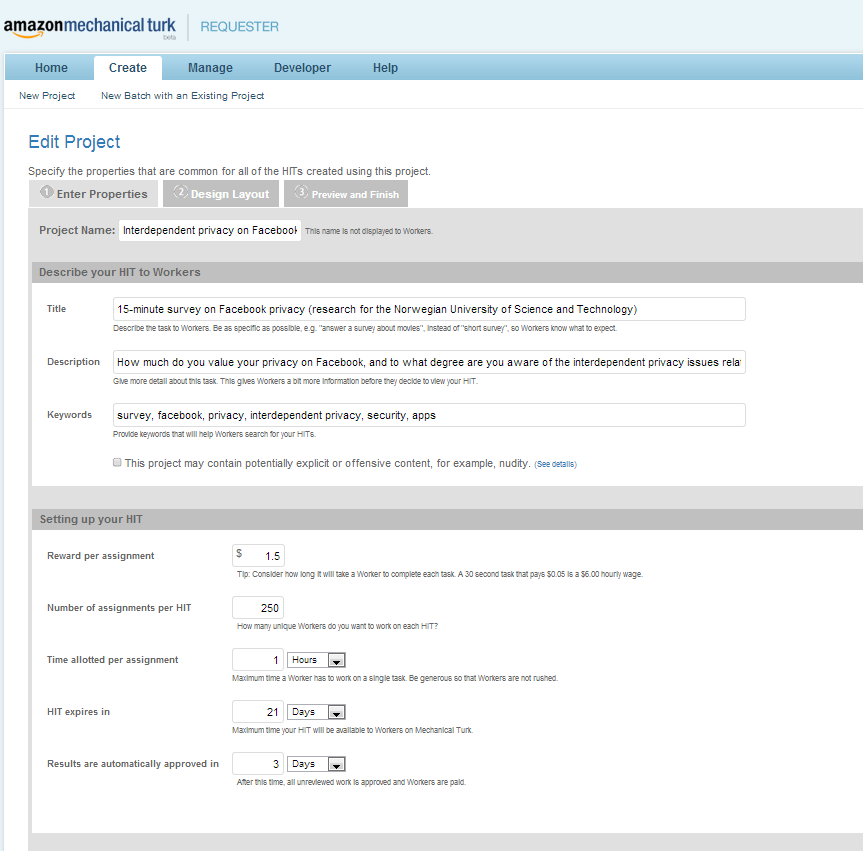
\includegraphics[width=1\textwidth]{amtedit.png} }
\caption[Creating an AMT project]{\textbf{Creating an AMT project.} This figure shows the layout for creating a new project in AMT. Here we stated the title, description, keywords, as well as defining the reward, number of unique workers and expiration date on the HIT.} 
\label{fig:amtedit}
\end{figure}

Next we filled in the "Survey-Link"-template provided by AMT, and the result of this is shown in \fref{fig:amtlayout}. It contains a title and a short description. In the description we linked to the homepage of the Norwegian University of Science and Technology, to emphasize the seriousness of the survey. In addition it contained the link to the survey on SurveyMonkey, as well as a field for the users to enter a survey code. This code was provided to them after they completed the survey. This was an assurance for us, so we only paid the people who actually took the survey. To avoid workers cheating with the code (for example getting the code from a fellow AMT-workers), we changed it several times during it's lifetime. 

\begin{figure}[h!]
\centering
\fbox{
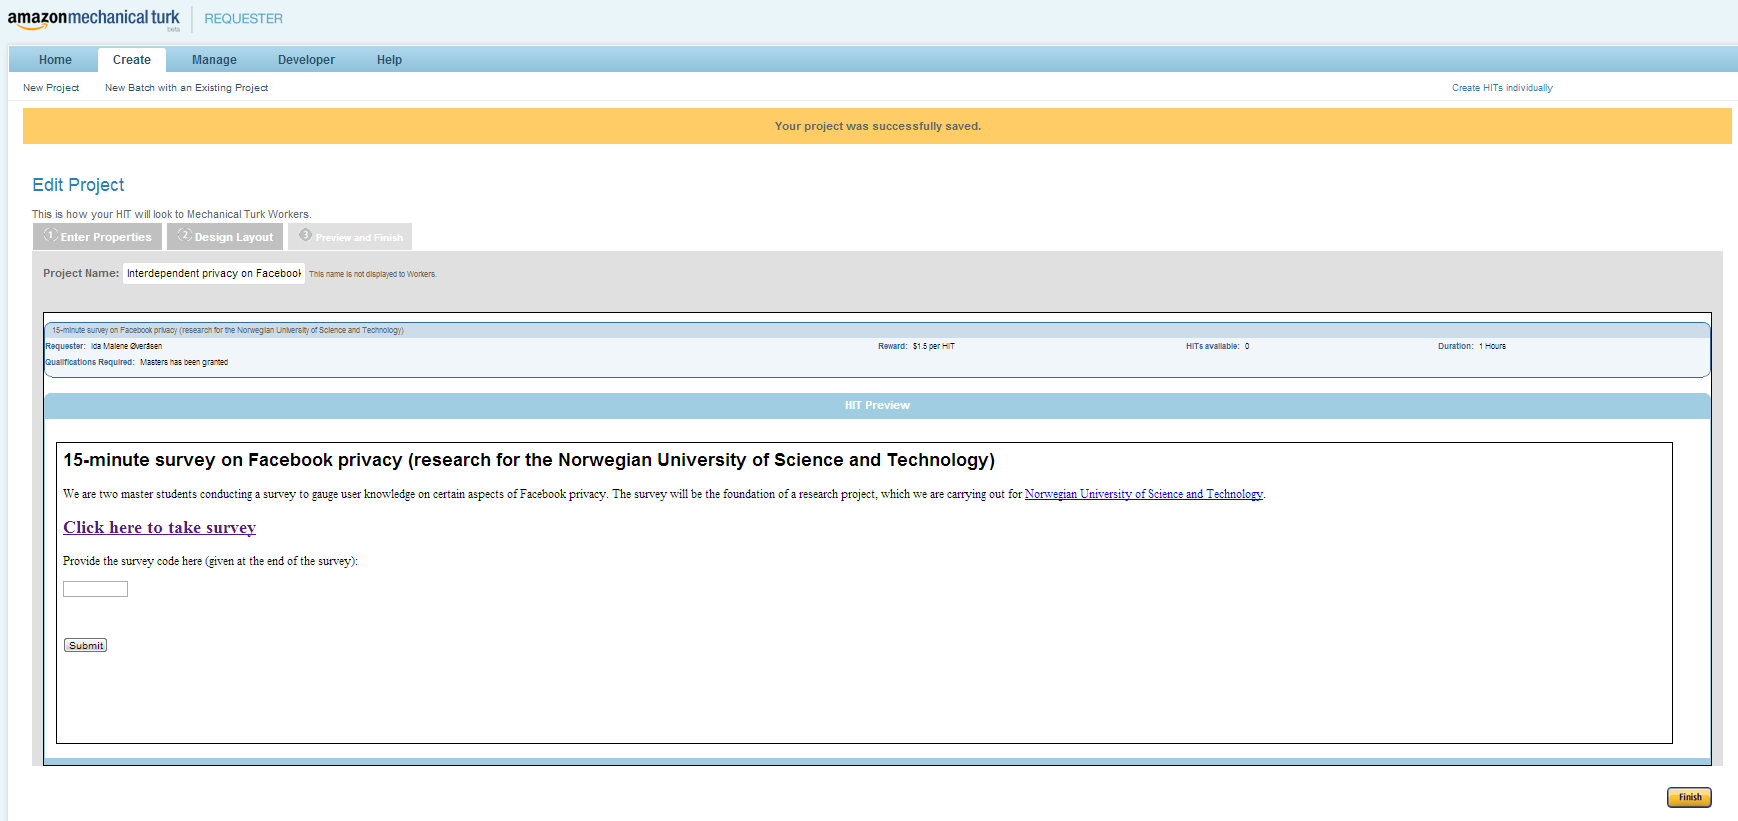
\includegraphics[width=1\textwidth]{amtlayout.png} }
\caption[The design and layout of the survey on AMT]{\textbf{The design and layout of the survey on AMT.} This figure shows the design and layout for the HIT. This is how it looks like for the workers.} 
\label{fig:amtlayout}
\end{figure}

After editing the project as described above, the HIT was ready to be published. The published HIT is shown in \fref{fig:hitout}. After filtering on HITs requiring Master qualification, our HIT is shown at the top. 
Once our HIT was out all we could do was monitor it (approve or discard answers), and wait for people to respond. 

\begin{figure}[h!]
\centering
\fbox{
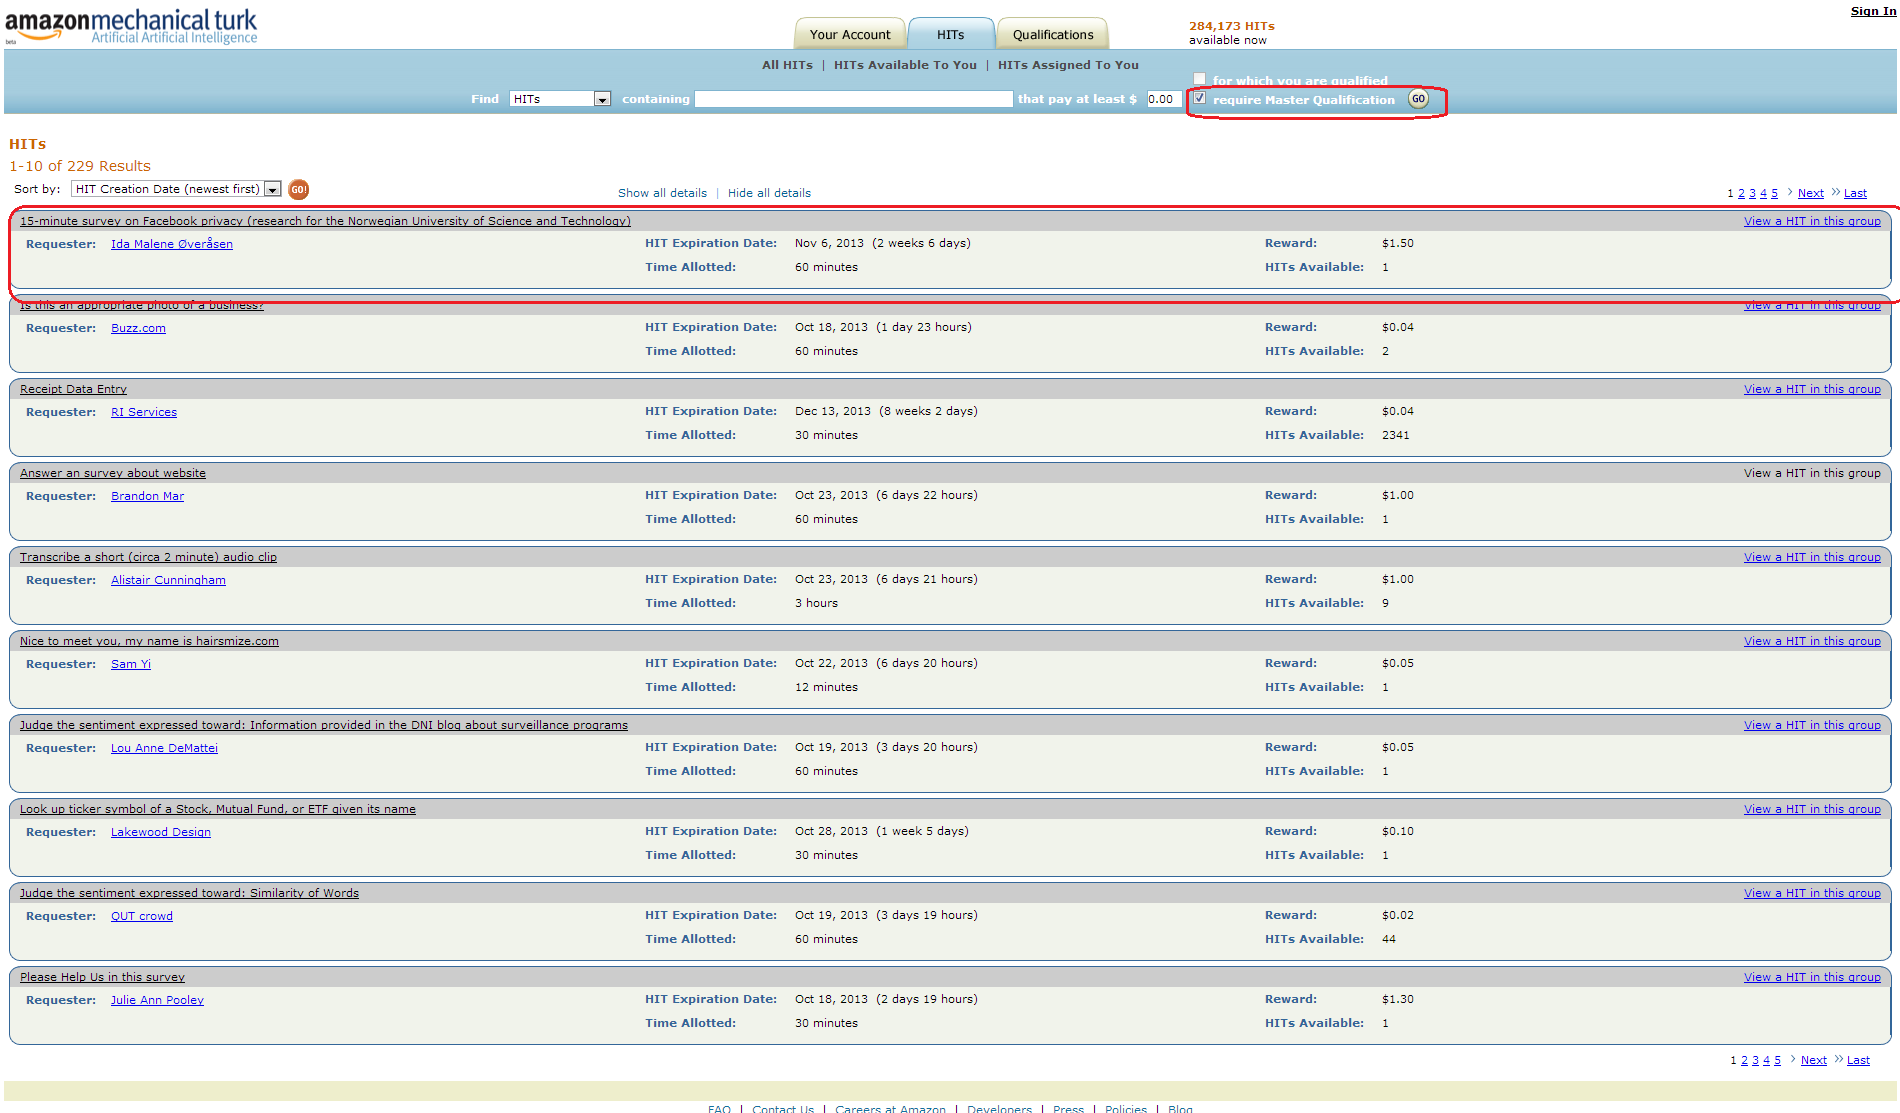
\includegraphics[width=1\textwidth]{hitout.png} }
\caption[Our HIT is published]{\textbf{Our HIT is published.} This figure shows our HIT in the list of all HITs available that requires "Master Workers".} 
\label{fig:hitout}
\end{figure}

We mainly wanted to distribute our survey on AMT, both to try it out as a research tool and because of it's high diversity. But in addition to distributing the survey on AMT, we decided to also share it with our friends on Facebook. We wanted to reach out to a even wider audience, as well as making our Facebook  friends aware of their settings. Most of our Facebook friends mainly consists of fellow students, with a high technical knowledge. We were not depending on Facebook to give us many answers. We were hoping for at least 30 respondents from Facebook, but we got 77 respondents and were amazed of the outcome. We posted it and a few times during the 3 weeks the survey was out, we commented on it so it would appear on top of our friends News Feeds. Three of our friends even chose to share it on their Facebook. This was probably one of the reasons we got so many answers. We posted it on Facebook a few days later than the HIT was published on AMT.  

\begin{figure}[h!]
\centering
\fbox{
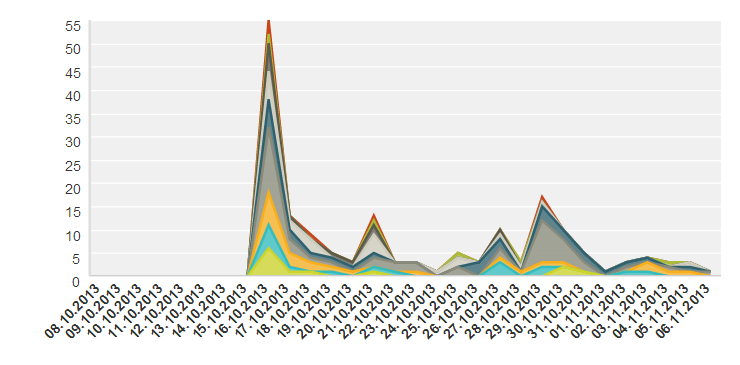
\includegraphics[width=1\textwidth]{answersamt.png} }
\caption[Daily distribution of number of answers from AMT]{\textbf{Daily distribution of number of answers from AMT.}} 
\label{fig:answersamt}
\end{figure}

\begin{figure}[h!]
\centering
\fbox{
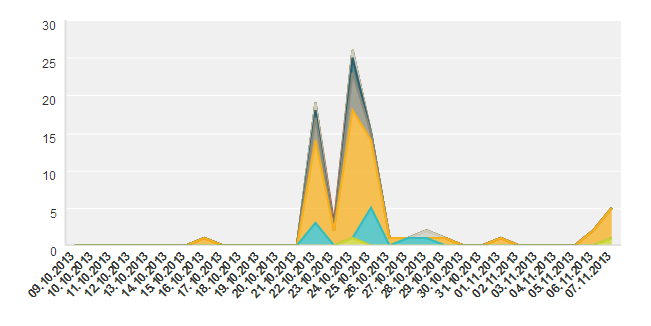
\includegraphics[width=1\textwidth]{answersfacebook.png} }
\caption[Daily distribution of number of answers from Facebook]{\textbf{Daily distribution of number of answers from Facebook.}} 
\label{fig:answersfacebook}
\end{figure}

\fref{fig:answersamt} and \fref{fig:answersfacebook} shows the daily distribution of number of answers, respectively from AMT and Facebook. You can see from \fref{fig:answersamt} that we had the highest peak in responses the day it was published. The first day we had 55 unique answers, and the second day it dropped to 13 answers. The number of responses varied during the rest of the period, as the figure shows. 

\subsection{Feedback on the Survey}
%citation i forum
%mange har kommentert at de åpna øynene litt etter å ha tatt den. 
%vi fikk likes og sånn







\section{Survey Results}
%Hvor mange svar vi fikk og sånn
%hvor lenge den lå ute på amt
%Hvordan vi har gått gjennom resultatene, hva vi har fokusert på og hvorfor!

\begin{figure}[h!]
\centering
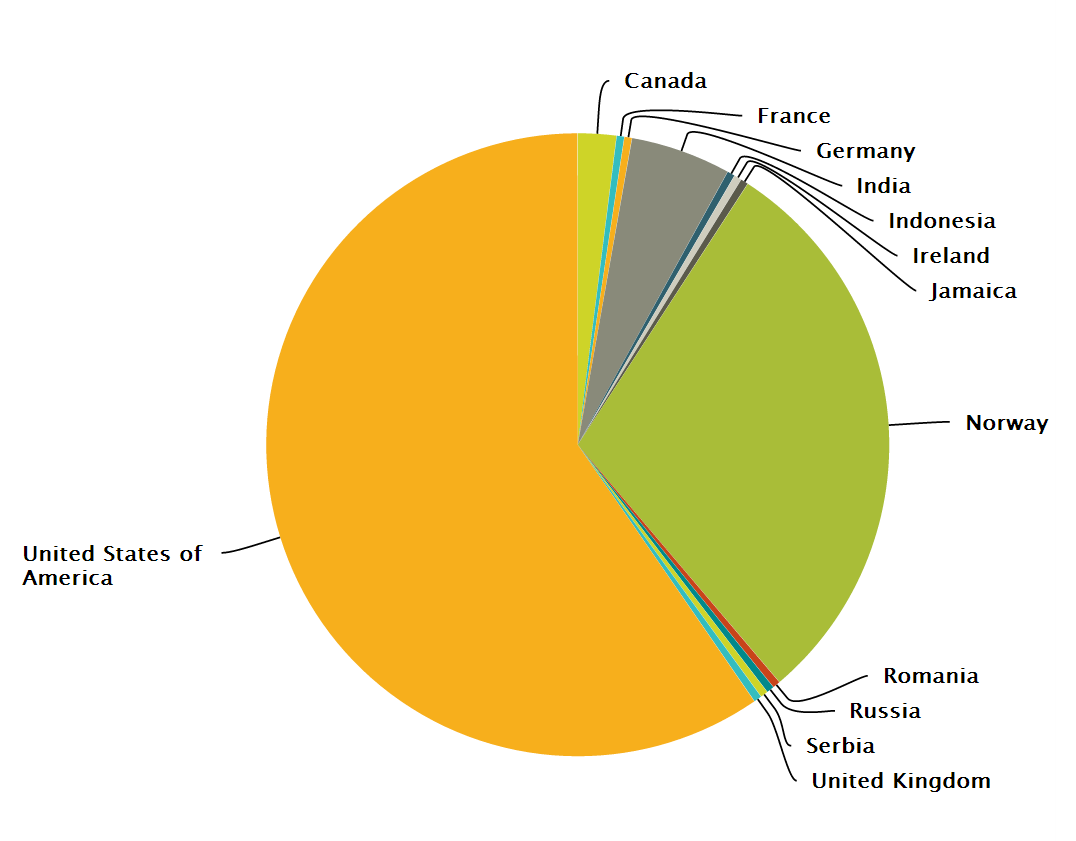
\includegraphics[width=1\textwidth]{land.png}
\caption[Distribution of the participant's country of origin]{\textbf{Distribution of the participant's country of origin.} This graph shows the distribution of the participant's country of origin. Most of the participants are from the United Stated of America and Norway.} 
\label{fig:land}
\end{figure}


\subsection{Demographics}

\begin{figure}[h!]
\centering
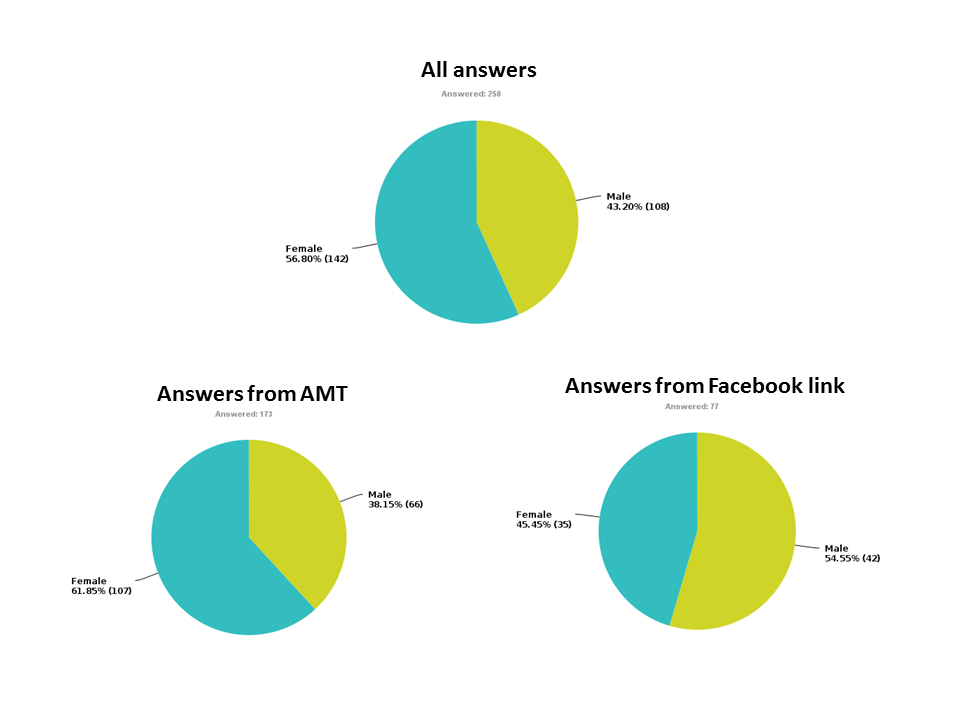
\includegraphics[width=1\textwidth]{gender.png}
\caption[Gender distribution]{\textbf{Gender distribution}. This graph shows the overall gender distribution (on the top), gender distribution from AMT (to the left) and the gender distribution from the Facebook link (to the right).} 
\label{fig:gender}
\end{figure}

As mentioned before we distributed our survey on two platforms; Amazon Mechanical Turk (AMT) and Facebook. As you can see in \fref{fig:land}, the distribution was mainly divided between two countries, the United States of America and Norway. Other countries are also represented; Canada, France, Germany, India, Indonesia, Ireland, Jamaica, Romania, Russia, Serbia and United Kingdom. 77 of the 250 responses were collected through the Facebook link, and out of these 77 people 96\% (74 people) are from Norway. 173 of the 250 respondents took the survey via Amazon Mechanical Turk, and out of these people 85,5\% (148 people) are from the United Stated of America. 

\paragraph{}
The majority of the total respondents were female. They accounted for 56,80\% of the responses, which is 142 responses. This means that 43,20\% of the total respondents were male, with a 108 responses. We saw a difference in the gender distribution from the Facebook link and from AMT. On AMT 38,15\% were men, and 56,80\% were female. On Facebook 54,55\% were male, and 45,55\% were female. In other word the majority of respondents on AMT were females, in contrary to Facebook, were the majority of respondents were men. The different gender distributions are shown in the \fref{fig:gender}.
 
\paragraph{}
Among the participants the age ranged betweetn 19 and 76. The average age is 31. The average age of the AMT participants (33 years old) are higher than the average age of the Facebook participants (27 years old). When we look at the total income of the household per year and employment status, we find a wide range of variety among the participants. We have several participants in each group of income. Although the majority of the participants are employed for wages or students, all of the other employment status' are represented. This is consistent with former studies of AMT users \cite{incentivesAmt}. 


\subsection{Frequency in Checking Facebook Privacy Settings}

\subsubsection{Never Checked Facebook Privacy Settings During the Last Year}

\begin{figure}[h!]
\centering
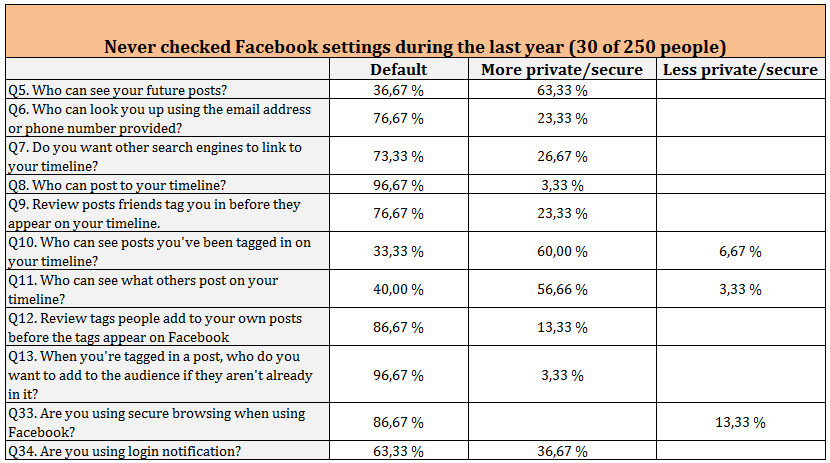
\includegraphics[width=1\textwidth]{nevercheckedtable.png}
\caption[Never checked Facebook privacy settings during the last year]{\textbf{Never checked Facebook privacy settings during the last year.} Forklare hva figuren viser.} 
\label{fig:neverchecked}
\end{figure}

30 of the people who answered our survey stated that they have never checked their privacy settings during the last year. Even though they have not checked their privacy settings during the last year, most of them have done some changes to their settings before the previous year. The reason for this assumption is that their settings differ from the default settings.  
The average number of friends for the people who have never checked Facebook privacy settings during the last year is 162, and their average age is 39. 

In \fref{fig:neverchecked} you can see a percentage distribution over Facebook settings among the people who have never checked their Facebook privacy settings during the last year. We have divided them into tree categories; "Default", "More secure", and "Less secure". You end up under the category "Default" if your settings is similar to the default settings anno 2013. See section \ref{subsec:default2013} for more detailed description of the default settings on Facebook. You end up under the "More secure" category if you have changed the default setting to a more secure settings. The "Less secure" is for those who have made changes to their settings which is less secure than the default settings. 

The majority of these users are active users, since 67\% of them checks their Facebook page at least once a day. 

60\% of the people who had never checked their Facebook privacy settings during the last year \textit{did not} consider changing their privacy settings after reviewing them. 40\% of them wanted to make their privacy settings more private. 

We have a quote from a 67 year old woman that took our survey (with Ph.D and only 5 Facebook friends) that emphasised many user's unawareness when it comes to different Facebook settings: "Now you have scared me. I am alone and afraid".


\subsubsection{Checks Facebook Privacy Settings "Once a month" or "Once a week or more"}

\begin{figure}[h!]
\centering
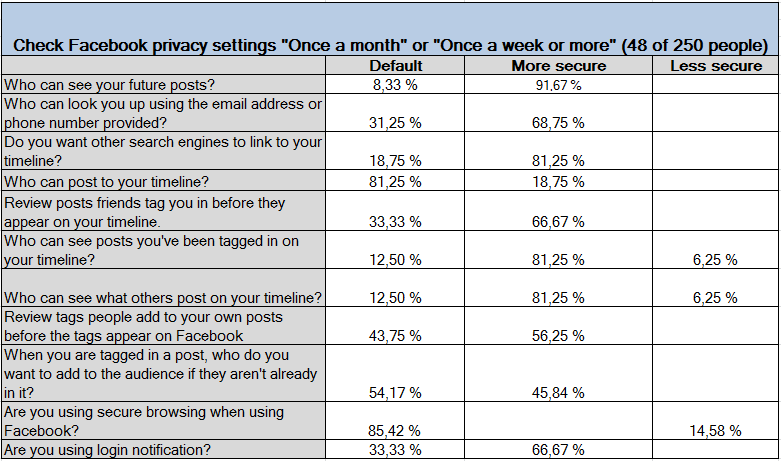
\includegraphics[width=1\textwidth]{checkonceaweekormoretable.png}
\caption[Checks Facebook privacy settings "Once a month" or "Once a week or more"]{\textbf{Checks Facebook privacy settings "Once a month" or "Once a week or more".} Forklare figuren mer nøye her} 
\label{fig:onceaweekormore}
\end{figure}

48 of the people who answered our survey stated that they check their privacy settings "Once a month" or "Once a week or more". The average number of friends for these people is 416, and their average age is 28,5. 

In \fref{fig:onceaweekormore} you can see a percentage distribution of what kind of settings the people who check their privacy settings "Once a month" or "Once a week or more" have. We have divided them into the same categories as above; "Default", "More secure", and "Less secure".  

85\% of the people who checked their Facebook privacy settings "Once a month" or "Once a week or more" during the last year, has checked their Facebook page at least once a day during the last month. This indicates that the majority of those who check their settings frequently are also very active Facebook users. 

70,83\% of these people did not consider changing privacy settings after reviewing them. 27,08 \% wanted to make their privacy settings more private, and 2,08\% considered changing them to more public. 


%12 of the 48 people in this category answered yes on the question whether or not facebook had affected their personal life negativally. Half of these had situations with friends posting unwanted pictures (av forskjellige grunner) of them.

%One guy: Two accounts; one under a pseudonym for friends only and on with strict settings for the rest of the world. "Privacy is important to me. It is meaningless not to give others the same courtesy" - Random guy with 420 friends that are 43 years old. 

\subsubsection{Comparing the ones Who Have Never Checked their Facebook Privacy Settings During the Last Year and the Ones Who Checks "Once a month" or "Once a week or more"} 

\paragraph{Activity level.}
The majority of both groups checks their Facebook page at least once a day. The percentage is a little bit higher for the people who have checked their privacy settings "Once a month" or "Once a week or more" during the last year. 85\% of them checks their Faceook page at least once a day, in contrast to the other group (who have never checked their settings during the last year) with 67\% checking their Facebook page at least once a day. This indicates that the ones who have never checked their settings during the last year does not refrain from doing this because they are inactive users. One assumption for this may be that the users are unaware of the settings. 40\% of them stated that they wanted to make their settings more private after taking the survey. This backs up the assumption about unawareness.  

\paragraph{More secure settings for those who check their settings more often?}
If we compare \fref{fig:neverchecked} and \fref{fig:onceaweekormore}, we see a clear difference in percentage that have changed from default to a more secure option. The percentage is much higher for all settings listed for those who checks frequently. Some of the settings shows a remarkable difference between the groups. We want to accentuate the settings that concern interdependent privacy. When we look at the setting "Review posts friends tag you in before they appear on your timeline" for the ones that never checked during the last year, only 23,33\% have changed to a more secure option. For the ones that check frequently, 66,67\% have changed to a more secure option. Another example is the setting "Review tags people add to you own posts before the tags appear on Facebook" where 13,33\% of the ones who never have checked their settings during the last year changed to a more secure option. On the contrary, as many as 56,25\% of the frequent settings-checkers have changed to a more secure option.

\paragraph{Considered changing settings.}
The percentage of those wanting to make their settings more private is higher for those who have never checked settings during the last year with 40\% of the group. Only 27\% of the frequent setting-checkers wanted to make their settings more private. 
None of the people who have never checked their settings during the last year wanted to make their settings more public, unlike the other group (those who check "Once a month" or "Once a week or more") where 2\% actually considered changing them to more public. Overall the frequent settings-checkers were more pleased with their settings than the once who had never checked them during the last year. 70\% of the frequent settings-checkers did not consider changing their settings after reviewing them. Although the ones who have never checked their settings during the last year have far less secure settings than the other group, 60\% of them did not consider changing their settings either. 


\subsection{Interdependent Privacy}
%finne ut på hvor mange som svarte ca. riktig på hva interdependent privacy er, første og siste gang. 


